\documentclass[11pt,a4paper]{article}

\usepackage[utf8]{inputenc}
\usepackage[T1]{fontenc}
\usepackage{lmodern}
\usepackage{microtype}
\emergencystretch=3em
\usepackage[margin=2.6cm]{geometry}
\usepackage{amsmath,amssymb,amsthm,mathtools}
\usepackage{booktabs,array}
\usepackage{enumitem}
\usepackage{tikz}
\usetikzlibrary{arrows.meta,positioning}
\usepackage[colorlinks=true,linkcolor=blue!50!black,citecolor=blue!50!black,urlcolor=blue!50!black]{hyperref}
\usepackage[capitalise,noabbrev]{cleveref}

\newtheorem{theorem}{Theorem}[section]
\newtheorem{lemma}[theorem]{Lemma}
\newtheorem{proposition}[theorem]{Proposition}
\newtheorem{corollary}[theorem]{Corollary}
\theoremstyle{definition}
\newtheorem{definition}[theorem]{Definition}
\theoremstyle{remark}
\newtheorem{remark}[theorem]{Remark}

\newcommand{\J}{\mathcal{J}}
\newcommand{\M}{\mathcal{M}}
\newcommand{\Minf}{\M^{\infty}}
\newcommand{\MP}{\M^{\mathrm{P}}}
\newcommand{\MU}{\M^{U}}
\newcommand{\Rel}{\mathcal{R}}
\newcommand{\Om}{\Omega}
\newcommand{\Cuts}{\mathcal{C}}
\newcommand{\Z}{\mathbb{Z}}
\newcommand{\R}{\mathbb{R}}
\newcommand{\code}[1]{\texttt{#1}}
\newcommand{\ind}[1]{\mathbf{1}[#1]}
\newcommand{\rc}{\bar c}
\newcommand{\RMP}{\mathrm{RMP}}

\title{The FED-HPC branch-price-and-cut solver:\\
mathematical formulation}
\author{fedhpc project notes}
\date{26 November 2026}

\begin{document}
\maketitle

\begin{abstract}
This note states the mathematics behind the exact branch-price-and-cut (BPC)
solver in \code{src/fedhpc/bpc.py} and its compiled pricer
\code{src/fedhpc/\_ext/bpc\_pricing.cpp}. We give the preprocessing that turns
an instance into path types and release groups, the Dantzig--Wolfe master
problem over instance-lifetime columns with all its optional rows (bound rows,
fixed-cost linking, activation rows and limited-memory subset-row cuts), its
dual, the reduced cost and its decomposition over arcs, the pricing problem
(an ng-route shortest path with resources on the space-time DAG of each type),
the Lagrangian bound, the stopping rules of column generation, reduced-cost
fixing, the branching rules and the way lexicographic and Pareto searches call
the solver. Each statement names the code that implements it.
\end{abstract}

\tableofcontents

%======================================================================
\section{Scope and notation}\label{sec:scope}
%======================================================================

The problem and its compact (space-time, arc-flow) model are those of the
note \code{formulation\_reductions.tex} in \code{docs/}; we reuse its notation and only recall
what is needed. The solver requires single-node jobs (it calls
\code{Instance.require\allowbreak\_unit\allowbreak\_demand}), so each job holds one instance of one
type for its whole processing time. The LP-first engine (\code{fedhpc.lpfirst})
for the large trace instances is a different method and is not covered here.

Time is discrete. A \emph{slot} $u\in\{0,\dots,H-1\}$ is the interval
$[u,u+1)$ and a \emph{node} $v\in\{0,\dots,H\}$ is an instant.

\paragraph{Data.}
\begin{itemize}[nosep]
  \item $\J$: jobs. Job $j$ has arrival $a_j$, release $r_j=\max(0,\lceil a_j\rceil)$
    and weight $w_j\ge0$ (an integer; \code{Instance.build} enforces this).
  \item $\M$: instance types. Type $m$ has capacity $N_m\in\Z_{\ge0}\cup\{\infty\}$
    and fixed usage cost $U_m\ge0$. $\MU:=\{m:U_m>0\}$.
  \item $F_j\subseteq\M$: types that fit job $j$. For $m\in F_j$: occupied time
    $p_{jm}\in\Z_{\ge1}$, cost $c_{jm}\ge0$ and feasible starts
    $T_{jm}=[r_j,H-p_{jm}]\cap\Z$.
  \item Running jobs: $\Rel^{\mathrm{run}}_m(v)$ instances of type $m$ become free
    at node $v\in\{1,\dots,H\}$ (a running job's clipped end), and
    $R_m=\sum_v \Rel^{\mathrm{run}}_m(v)$ instances are busy at $0$.
  \item Cost resolution $\delta>0$: every $c_{jm}$ and $U_m$ is an integer
    multiple of $\delta$ (\code{c\_units}).
\end{itemize}

\paragraph{Schedules and objectives.} A schedule assigns each job a type
$\mu_j\in F_j$ and a start $s_j\in T_{j\mu_j}$, with completion
$C_j=s_j+p_{j\mu_j}$. It is feasible if at every slot at most $N_m$ instances of
type $m$ are busy (running jobs included). The objectives are
\[
f_1=\sum_{j\in\J} w_j\,(C_j-a_j),\qquad
f_2=\sum_{j\in\J} c_{j\mu_j}+\sum_{m\in\mu(\J)}U_m .
\]

\paragraph{The problem the tree solves.} Every call of
\code{\_branch\_and\_price} solves
\begin{equation}\label{eq:P}
\tag{P}
z^\star(\omega,B)=\min\bigl\{\omega_1 f_1+\omega_2 f_2 \;:\;
\text{feasible schedule},\ f_1\le B_1,\ f_2\le B_2\bigr\},
\end{equation}
with $\omega_1,\omega_2\ge0$ (\code{weight1}, \code{weight2}) and optional caps
$B_1,B_2\in\R\cup\{+\infty\}$ (\code{bound1\_value}, \code{bound2\_value}).
A missing cap means the row is not built. Lexicographic and Pareto searches are
sequences of such calls (\cref{sec:lex}).

%======================================================================
\section{Preprocessing}\label{sec:prep}
%======================================================================

\code{\_prepare} computes the following once per instance. A Pareto search
shares the result across all its box solves.

\subsection{Reduced start sets}
If the data are nonnegative ($w_j,c_{jm},U_m\ge0$), the start sets are reduced
to $S_{jm}\subseteq T_{jm}$ by the objective-independent exact reductions of
\code{formulations}: normal-pattern starts (N1), the collapse of unbounded
types to their release (R1) and the Pareto filter on unbounded options (R2).
Otherwise $S_{jm}=T_{jm}$. Pairs with $S_{jm}=\emptyset$ are dropped. These
reductions never raise $f_1$ or $f_2$ of any schedule (proofs in
\code{docs/formulation\_reductions.tex}), so they remain valid under both caps
of \eqref{eq:P} and under any branching decision. The objective-dependent
reductions R3 and LX are not valid under an $f_2$ cap and are not used.

\subsection{Unbounded types and path types}
A type is \emph{unbounded} if its capacity can never bind:
\[
\Minf := \bigl\{m\in\M : N_m=\infty \ \text{ or }\ N_m-R_m\ \ge\ |\{j: m\in F_j\}|\bigr\}
\]
(\code{formulations.unbounded\_types}). On such a type every job may run on
its own instance, so a multi-job timeline is never needed: it splits into
single-job timelines with the same total cost. The remaining types are the
\emph{path types} $\MP:=\M\setminus\Minf$.

\subsection{Release groups}
For $m\in\MP$ the instances are grouped by the node at which they become free
(\code{\_release\_classes}):
\[
N_{m,0}:=N_m-R_m,\qquad N_{m,r}:=\Rel^{\mathrm{run}}_m(r)\quad(1\le r<H),
\]
and $\Rel_m:=\{r: N_{m,r}>0\}$. An instance released at $H$ can run nothing and
is left out. Each group $(m,r)$ gets its own fleet row
(\cref{sec:master}), which reproduces the compact model's boundary condition
$y_{m,-1}=N_m-R_m$ together with the running-job inflows $\Rel^{\mathrm{run}}_m(v)$.

%======================================================================
\section{Columns}\label{sec:columns}
%======================================================================

\subsection{The space-time network of a path type}
For $m\in\MP$, the network $G_m$ has nodes $\{0,\dots,H\}$, a wait arc
$(v,v+1)$ for every $v<H$, and a \emph{processing arc} $(j,t)$ from $t$ to
$t+p_{jm}$ for every $j$ with $m\in F_j$ and $t\in S_{jm}$. It is a DAG ordered
by time.

\begin{figure}[ht]
\centering
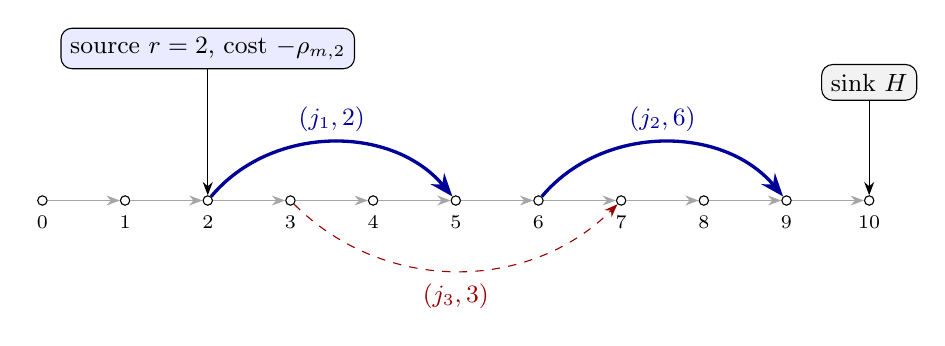
\begin{tikzpicture}[x=1.05cm,y=1cm,>=Stealth]
  \foreach \v in {0,...,10} {
    \node[circle,draw,inner sep=1.2pt,fill=white] (n\v) at (\v,0) {};
    \node[below=2pt] at (\v,0) {\scriptsize $\v$};
  }
  \foreach \v [evaluate=\v as \w using int(\v+1)] in {0,...,9}
    \draw[->,gray!70] (n\v) -- (n\w);
  \draw[->,very thick,blue!60!black] (n2) to[bend left=50] node[above]{\small $(j_1,2)$} (n5);
  \draw[->,very thick,blue!60!black] (n6) to[bend left=50] node[above]{\small $(j_2,6)$} (n9);
  \draw[->,dashed,red!60!black] (n3) to[bend right=45] node[below=1pt]{\small $(j_3,3)$} (n7);
  \node[draw,rounded corners,fill=blue!8,above=1.6cm of n2,anchor=south] (src) {\small source $r=2$, cost $-\rho_{m,2}$};
  \draw[->] (src) -- (n2);
  \node[draw,rounded corners,fill=gray!10] (snk) at (10,1.5) {\small sink $H$};
  \draw[->] (snk) -- (n10);
\end{tikzpicture}
\caption{A column of release group $(m,2)$ in $G_m$ with $H=10$: wait to $2$,
run $j_1$ on $[2,5)$, wait, run $j_2$ on $[6,9)$, wait to $H$. The dashed arc
is another processing arc of $G_m$ that this column does not use.}
\label{fig:network}
\end{figure}

\begin{definition}[Path column]\label{def:column}
A column of release group $(m,r)$, $m\in\MP$, $r\in\Rel_m$, is a sequence
$p=\bigl((j_1,t_1),\dots,(j_k,t_k)\bigr)$, $k\ge0$, of processing arcs of $G_m$
with
\[
r\le t_1,\qquad t_i+p_{j_im}\le t_{i+1}\ (1\le i<k),\qquad t_k+p_{j_km}\le H .
\]
It is one instance's timeline over the whole horizon (a source-to-sink path in
$G_m$ from node $r$, with waits filled in). The empty sequence is the
\emph{null column} $\emptyset_{m,r}$ (an idle instance). The column is
\emph{elementary} if $j_1,\dots,j_k$ are distinct. Its data are
\begin{align*}
a_{jp}&:=|\{i: j_i=j\}| &&\text{(visit count of job $j$)},\\
c^1_p&:=\textstyle\sum_{i=1}^k w_{j_i}\,(t_i+p_{j_im}-a_{j_i}) &&\text{(its share of $f_1$)},\\
c^2_p&:=\textstyle\sum_{i=1}^k c_{j_im} &&\text{(its share of $f_2$ without $U_m$)}.
\end{align*}
$\Om_{m,r}$ is the set of columns the pricer may generate for group $(m,r)$
(\cref{sec:ng}): all elementary columns, plus some that repeat a job.
$\Om_m:=\bigcup_{r}\Om_{m,r}$.
\end{definition}

\begin{definition}[Static column]
For $m\in\Minf$, $m\in F_j$ and $t\in S_{jm}$, the \emph{static column}
$q=(j,m,t)$ is the single-job timeline with $a_{jq}=1$,
$c^1_q=w_j(t+p_{jm}-a_j)$ and $c^2_q=c_{jm}$. $\Om^\infty_j$ denotes the static
columns of job $j$ and $\Om^\infty:=\bigcup_j\Om^\infty_j$. They are all
enumerated up front (\code{static\_columns}); under R1 each pair $(j,m)$ has
one start, so there are at most $|\J|\,|\Minf|$ of them.
\end{definition}

%======================================================================
\section{The master problem}\label{sec:master}
%======================================================================

\subsection{Variables}
\begin{itemize}[nosep]
  \item $\lambda_p\ge0$ for every path column $p\in\Om_{m,r}$: the number of
    instances of group $(m,r)$ following timeline $p$.
  \item $\lambda_q\ge0$ for every static column $q\in\Om^\infty$.
  \item $z_m\in[0,1]$ for $m\in\MU$: type $m$ is used.
  \item $\alpha_j\ge0$ for $j\in\J$: an artificial variable with cost $\bar M$
    (\code{\_big\_m\_for}: $10^6$ times the largest of the cost, fixed-cost and
    $H\cdot\max_j w_j$ scales). It keeps every restricted master LP feasible
    before columns cover all jobs.
  \item Cuts: a finite set $\Cuts$ of limited-memory subset-row cuts
    (\cref{sec:cuts}), each with coefficients $\gamma_c(p)\in\Z_{\ge0}$.
\end{itemize}

\subsection{The master LP}
Write $\Om^{\mathrm P}:=\bigcup_{m\in\MP}\Om_m$ for all path columns and
$c^\omega_v:=\omega_1c^1_v+\omega_2c^2_v$ for the cost of a column $v$. The
master LP over all columns, with the dual variable of each row on the right,
is
\begin{alignat}{3}
\min\quad & \sum_{p\in\Om^{\mathrm P}}c^\omega_p\lambda_p
 +\sum_{q\in\Om^\infty}c^\omega_q\lambda_q
 +\omega_2\sum_{m\in\MU}U_m z_m+\bar M\sum_{j\in\J}\alpha_j \notag\\
\text{s.t.}\quad
& \sum_{p\in\Om^{\mathrm P}} a_{jp}\lambda_p+\sum_{q\in\Om^\infty_j}\lambda_q+\alpha_j = 1
  &\;& j\in\J &\;& [\sigma_j] \label{eq:cover}\\
& \sum_{p\in\Om_{m,r}}\lambda_p = N_{m,r}
  && m\in\MP,\ r\in\Rel_m && [\rho_{m,r}] \label{eq:fleet}\\
& \sum_{p\in\Om^{\mathrm P}}c^1_p\lambda_p+\sum_{q\in\Om^\infty}c^1_q\lambda_q \le B_1
  && \text{if } B_1<\infty && [\nu_1\le0] \label{eq:b1}\\
& \sum_{p\in\Om^{\mathrm P}}c^2_p\lambda_p+\sum_{q\in\Om^\infty}c^2_q\lambda_q+\sum_{m\in\MU}U_mz_m \le B_2
  && \text{if } B_2<\infty && [\nu_2\le0] \label{eq:b2}\\
& \sum_{p\in\Om_m}a_{jp}\lambda_p+\sum_{q\in\Om^\infty_{jm}}\lambda_q - z_m\le 0
  && m\in\MU\cap F_j && [\theta_{jm}\le0] \label{eq:link}\\
& \sum_{p\in\Om_m\setminus\{\emptyset\}}\lambda_p - N^{\mathrm{P}}_m z_m\le 0
  && m\in\MU\cap\MP && [\eta_m\le0] \label{eq:act}\\
& \sum_{p\in\Om^{\mathrm P}}\gamma_c(p)\lambda_p\le 1
  && c\in\Cuts && [\beta_c\le0] \label{eq:cut}\\
& \lambda\ge0,\quad \alpha\ge0,\quad \ell_m\le z_m\le u_m\ \ (m\in\MU), \notag
\end{alignat}
where $N^{\mathrm{P}}_m:=\sum_{r\in\Rel_m}N_{m,r}$ is the number of instances of
path type $m$ that can do work, $\Om^\infty_{jm}$ is the set of static
columns of $j$ on type $m$, and $[\ell_m,u_m]=[0,1]$ unless a branching
decision fixes $z_m$ (\cref{sec:branch}). The duals $\sigma_j$ and
$\rho_{m,r}$ of the equality rows are free.

\paragraph{Row by row} (\code{\_build\_rmp}, \code{\_add\_column\_var}).
\begin{itemize}[leftmargin=*]
\item \eqref{eq:cover} \emph{Coverage.} Each job is processed once. A column that
  repeats a job has its visit count as coefficient, so it can never take part
  in an integer solution.
\item \eqref{eq:fleet} \emph{Fleet.} Exactly $N_{m,r}$ timelines start at $r$;
  idle instances take the null column, which is seeded in every master so
  pricing never has to find it. Unbounded types have no fleet row.
\item \eqref{eq:b1}--\eqref{eq:b2} \emph{Bound rows.} Aggregate caps on $f_1$ and
  $f_2$; both may be present at once. $z_m$ enters the $f_2$ row with
  coefficient $U_m$ (it never enters the $f_1$ row).
\item \eqref{eq:link} \emph{Fixed-cost linking.} The master copy of the compact
  model's $\sum_t x_{jmt}\le z_m$, one row per $(j,m)$ (disaggregated, as in
  the compact model). The coefficient of a column is again the visit count.
\item \eqref{eq:act} \emph{Activation rows} (built only with the compiled pricer).
  At most $N^{\mathrm{P}}_m$ non-null timelines of $m$, and none unless $z_m=1$.
  It is valid for every integer solution. When $N^{\mathrm{P}}_m=1$ (the Rm
  machines) it charges $U_m$ to the column itself, as in the master of Chen
  and Powell~\cite{chen1999}, which \eqref{eq:link} alone does not: there a
  column pays $U_m$ only in proportion to its largest single-job share.
\item \eqref{eq:cut} \emph{Limited-memory subset-row cuts} (off by default;
  \cref{sec:cuts}).
\end{itemize}

A \emph{restricted master} $\RMP$ keeps a finite subset of the path columns
(all static columns, the null columns, heuristic seed columns and those found
by pricing). Each B\&B node builds its own $\RMP$ from scratch, seeded with the
parent's columns that survive the node's decisions (\code{\_column\_allowed});
columns that repeat a job are not inherited.

\subsection{Integer master and schedules}

\begin{proposition}\label{prop:integer}
Let $\Om_{m,r}$ contain all elementary columns. Then
\begin{enumerate}[label=(\alph*),nosep]
\item every solution of \eqref{eq:cover}--\eqref{eq:cut} with $\alpha=0$,
  $\lambda$ integer and $z$ binary uses only elementary columns and induces a
  feasible schedule within the caps $B_1,B_2$, with objective
  $\omega_1f_1+\omega_2f_2$ at most the master objective;
\item conversely every feasible schedule that respects the caps and uses
  starts in $S_{jm}$ has such a master solution with the same objective.
\end{enumerate}
Hence the integer master with columns $\Om$ solves \eqref{eq:P} restricted to
the reduced start sets, which by \cref{sec:prep} has the same optimal value as
\eqref{eq:P}.
\end{proposition}

\begin{proof}
(a) By \eqref{eq:cover} with $\alpha=0$ and integer $\lambda$, each job $j$
lies in exactly one selected column and is visited once in it, so the selected
columns are elementary in $j$ and define $(\mu_j,s_j)$. On $m\in\MP$, the
selected columns of group $(m,r)$ number $N_{m,r}$ by \eqref{eq:fleet}; each is
a sequence of non-overlapping intervals after $r$, so at any slot $u$ at most
$\sum_{r\le u}N_{m,r}$ jobs run on $m$, which is $N_m$ minus the running jobs
still busy at $u$. So capacity holds. Types in $\Minf$ cannot violate capacity
by definition. The column costs add up to $f_1$ and to $f_2$ without fixed
costs. If a job uses $m\in\MU$, then \eqref{eq:link} forces $z_m=1$, so the
master pays at least $\sum_{m\in\mu(\J)}U_m$, and \eqref{eq:b2} holds with the
true $f_2$ on its left. (b) For each path type, assign the jobs in order of
start to the instance that became free latest among those free by the start
(interval partitioning, \code{\_schedule\_columns}). An instance free at a job's
start stays free for every later one, so a capacity-feasible schedule always
fits, and each instance's sequence is an elementary column of its group; idle
instances get the null column. Jobs on unbounded types take their static
column, and $z_m:=\ind{m\in\mu(\J)}$. All rows hold, \eqref{eq:act} because
at most $N^{\mathrm P}_m$ instances do work.
\end{proof}

%======================================================================
\section{Reduced cost and its decomposition}\label{sec:rc}
%======================================================================

Let $d=(\sigma,\rho,\nu,\theta,\eta,\beta)$ be a dual vector with the signs
of \cref{sec:master}. Absent rows have dual $0$; write $\theta_{jm}:=0$ for
$m\notin\MU$ and $\eta_m:=0$ for $m\notin\MU$.

\paragraph{Path columns} (\code{\_column\_rc}). For $p\in\Om_{m,r}$,
\begin{equation}\label{eq:rc}
\rc_p(d)=(\omega_1-\nu_1)c^1_p+(\omega_2-\nu_2)c^2_p
-\sum_{j}a_{jp}\,(\sigma_j+\theta_{jm})
-\eta_m\,\ind{p\ne\emptyset}
-\sum_{c\in\Cuts}\beta_c\,\gamma_c(p)
-\rho_{m,r}.
\end{equation}
For $p=\bigl((j_i,t_i)\bigr)_{i=1}^k$ every term but the last three is a sum
over arcs. With
\begin{align}
B_{jm}&:=(\omega_1-\nu_1)\,w_j, \label{eq:B}\\
A_{jm}&:=(\omega_1-\nu_1)\,w_j\,(p_{jm}-a_j)+(\omega_2-\nu_2)\,c_{jm}-\sigma_j-\theta_{jm}, \label{eq:A}
\end{align}
the processing arc $(j,t)$ costs $A_{jm}+B_{jm}\,t$, and
\begin{equation}\label{eq:rc-decomp}
\rc_p(d)=\underbrace{-\rho_{m,r}}_{\text{source}}
+\underbrace{\kappa^{\eta}_m\,\ind{k\ge1}}_{\text{first arc}}
+\sum_{i=1}^k\bigl(A_{j_im}+B_{j_im}\,t_i\bigr)
+\underbrace{\sum_{c\in\Cuts}\kappa_c\,\gamma_c(p)}_{\text{cut states}}
\end{equation}
with $\kappa^\eta_m:=-\eta_m\ge0$ and $\kappa_c:=-\beta_c\ge0$
(\code{\_NodePricing.\_inputs} builds $A$, $B$ and the source costs). Wait arcs cost nothing. Since
$\nu_1\le0$, $B_{jm}\ge0$, but the pricer does not rely on it.

\paragraph{Other variables.}
\begin{align*}
\rc_q(d)&=(\omega_1-\nu_1)c^1_q+(\omega_2-\nu_2)c^2_q-\sigma_j-\theta_{jm}
  && q=(j,m,t)\in\Om^\infty,\\
\rc_{\alpha_j}(d)&=\bar M-\sigma_j,\\
\rc_{z_m}(d)&=(\omega_2-\nu_2)\,U_m+\sum_{j:m\in F_j}\theta_{jm}+N^{\mathrm P}_m\,\eta_m
  && m\in\MU.
\end{align*}

%======================================================================
\section{Pricing}\label{sec:pricing}
%======================================================================

For each path type $m\in\MP$ and each node, the pricing problem is
\begin{equation}\label{eq:pricing}
\rc^\star_m(d):=\min\bigl\{\rc_p(d) : p\in\Om_{m,r},\ r\in\Rel_m,\
p \text{ allowed by the node's decisions}\bigr\},
\end{equation}
one problem per type over all its release groups at once. It is a shortest
path on the DAG $G_m$ with one source per group, made hard by the job-repeat
restriction, the Ryan--Foster pairs and the cut states. The compiled pricer
(\code{Pricer::run}) solves it by label setting; the Python pricer
(\code{\_price\_type}) is the elementary reference implementation.

\subsection{ng-route relaxation}\label{sec:ng}
Each job $i$ on type $m$ has a \emph{neighbourhood} $N_i\subseteq\J$ with
$i\in N_i$ (\code{\_ensure\_ng}): $i$ and the $\texttt{ng\_size}-1$ jobs
closest to it in the score $|\,\bar t_i-\bar t_{i'}\,|+|\,p_{im}-p_{i'm}|$,
where $\bar t_i=(\min S_{im}+\max S_{im}+p_{im})/2$ is the centre of $i$'s
window. Jobs of a Ryan--Foster pair are added to every neighbourhood.

A partial path carries a \emph{memory} $\Pi\subseteq\J$. Extending by job $i$ is
allowed only if $i\notin\Pi$, and then
\[
\Pi\ \leftarrow\ (\Pi\cap N_i)\cup\{i\}.
\]
$\Om_{m,r}$ is the set of ng-feasible paths
(Baldacci, Mingozzi and Roberti~\cite{baldacci2011}). It contains every
elementary path, and with $N_i=\J$ for all $i$ it is exactly the elementary
set (\code{ng\_size=None}). A column of $\Om_{m,r}$ may repeat a job $j$ only
if some job between the two visits does not remember $j$.

\paragraph{Dynamic neighbourhoods} (\code{\_augment\_ng}, \code{\_grow\_ng\_and\_drop};
Roberti and Mingozzi~\cite{roberti2014}). When column generation has converged
and the LP uses a column that repeats a job $j$ at positions $a<b$, the job
$j$ is added to $N_i$ for every job $i$ at a position strictly between $a$ and
$b$ (up to $|N_i|<\texttt{ng\_max}$). That cycle is then infeasible. Every
repeating column leaves the $\RMP$ and generation resumes. This stops when the
converged LP is elementary or no neighbourhood can grow.

\subsection{Labels}
A label at node $t$ is $\ell=(t,\ c_\ell,\ \Pi_\ell,\ \pi_\ell,\ s_\ell)$ where
\begin{itemize}[nosep]
\item $c_\ell$ is the reduced cost so far;
\item $\Pi_\ell$ is the ng memory (a bitset over the type's jobs);
\item $\pi_\ell\in\{0,1\}^{\mathcal{S}}$ is the parity vector of the node's
  Ryan--Foster \emph{same} pairs $\mathcal S$ (bit $s$ flips when either job of
  pair $s$ is visited);
\item $s_\ell\in\{0,1\}^{\Cuts}$ is the state vector of the subset-row cuts.
\end{itemize}
For each $r\in\Rel_m$ there is a source label $(r,-\rho_{m,r},\emptyset,0,0)$.

\paragraph{Extension} along processing arc $(i,t)$, $t\in S_{im}$ allowed at
this node, from a label $\ell$ at node $t$ (the label is available at every
node from its own on, so wait arcs are implicit). It is feasible if
$i\notin\Pi_\ell$ and no Ryan--Foster \emph{differ} partner of $i$ is in
$\Pi_\ell$. The new label at node $t+p_{im}$ has
\begin{align*}
c'&=c_\ell+A_{im}+B_{im}\,t+\kappa^\eta_m\,\ind{\ell\text{ is a source label}}
   +\sum_{c\in\Cuts:\ i\in S_c,\ \hat s_{\ell,c}=1}\kappa_c,\\
\Pi'&=(\Pi_\ell\cap N_i)\cup\{i\},\qquad
\pi'=\pi_\ell\oplus\tau_i,\qquad
s'_c=\hat s_{\ell,c}\oplus\ind{i\in S_c},
\end{align*}
where $\tau_i$ flags the same pairs containing $i$, and
$\hat s_{\ell,c}=s_{\ell,c}\,\ind{i\in M_c}$ is the cut state after the reset
rule of \cref{sec:cuts}. A label is a \emph{complete column} at any node if
$\pi_\ell=0$ (each same pair has both jobs or neither); its reduced cost is
$c_\ell$, because waiting to $H$ is free.

\paragraph{Dominance.} $\ell_1$ dominates $\ell_2$ (\code{Arena::dom}) if
\[
c_{\ell_1}+\kappa^\eta_m\,\ind{\ell_1\text{ source},\ \ell_2\text{ not}}
+\sum_{c:\ s_{\ell_1,c}=1,\ s_{\ell_2,c}=0}\kappa_c\ \le\ c_{\ell_2},
\qquad \Pi_{\ell_1}\subseteq\Pi_{\ell_2},\qquad \pi_{\ell_1}=\pi_{\ell_2},
\]
and $\ell_1$ is available no later than $\ell_2$. Every extension of $\ell_2$
is then feasible from $\ell_1$, at a cost no greater: $\ell_1$ pays each cut it
has armed and $\ell_2$ has not at most once more. Labels are kept per node in
a cost-sorted \emph{active set}, and a label created at node $t$ joins it at
$t$; there are no copies along wait arcs and no bucket cap.

\subsection{Completion bound and exactness}
Define the cheapest completion from node $t$ with repeats allowed and no
first-arc or cut cost:
\begin{equation}\label{eq:g}
g(H)=0,\qquad g(t)=\min\Bigl\{g(t+1),\ \min_{i:\,t\in S_{im}}\bigl(A_{im}+B_{im}t+g(t+p_{im})\bigr)\Bigr\}.
\end{equation}
Because $\kappa^\eta_m,\kappa_c\ge0$, every completion of a label $\ell$ at $t$
costs at least $c_\ell+g(t)$. With threshold $\vartheta=-\texttt{tol}$, a label
with $c_\ell+g(t)\ge\vartheta$ is retired, and an extension with
$c'+g(t+p_{im})\ge\vartheta$ is not built. The active set is scanned cheapest
first, so for a fixed arc the scan stops at the first label with
$c_\ell+A_{im}+B_{im}t+g(t+p_{im})\ge\vartheta$; all later labels fail too.

The pricer returns
\[
\underline{\rc}_m:=\min\bigl\{\text{best complete label},\ \text{every retired or skipped bound } c+g\bigr\}
\ \le\ \rc^\star_m(d),
\]
which is the exact minimum when that minimum is below $\vartheta$, and the
\texttt{cols\_per\_type} cheapest distinct complete labels below $\vartheta$
as new columns. If the label budget \texttt{max\_labels} runs out, the call
is marked inexact and gives no bound.

\paragraph{Early stop in the plain case.} Without same pairs and without cuts,
$\pi=s=0$ for every label. A stored extension by job $i$ from a non-source
label with memory $\{i\}$ then dominates all costlier candidates of the same
arc, and the scan stops there.

%======================================================================
\section{Lagrangian bound}\label{sec:lagr}
%======================================================================

\begin{proposition}[\code{\_lagrangian\_bound}]\label{prop:lagr}
Let $d$ be any dual vector with $\nu_1,\nu_2,\theta,\eta,\beta\le0$ (not
necessarily optimal for the $\RMP$), and let $\underline{\rc}_m\le\rc^\star_m(d)$
for every $m\in\MP$. Then the master LP value at the node is at least
\begin{align}
L(d)={}&\sum_{j}\sigma_j+\sum_{m\in\MP}\sum_{r\in\Rel_m}N_{m,r}\,\rho_{m,r}
+\nu_1B_1+\nu_2B_2+\sum_{c\in\Cuts}\beta_c \notag\\
&+\sum_{m\in\MP}N^{\mathrm P}_m\,\underline{\rc}_m
+\sum_{j}\min\Bigl\{0,\ \bar M-\sigma_j,\ \min_{q\in\Om^\infty_j}\rc_q(d)\Bigr\}
+\sum_{m\in\MU}\rc_{z_m}(d)\cdot\begin{cases}\ell_m&\rc_{z_m}\ge0\\ u_m&\rc_{z_m}<0\end{cases}.
\label{eq:lagr}
\end{align}
\end{proposition}

\begin{proof}
For any feasible master solution, the objective equals $d^\top b$ plus
$\sum_v \rc_v(d)\,v$ minus the slack of each inequality row times its dual.
Those slacks are $\ge0$ and their duals are $\le0$, so the objective is at
least $d^\top b+\sum_v\rc_v v$, where $d^\top b$ is the first line of
\eqref{eq:lagr} (absent bound rows contribute $0$). For path columns, the
$\lambda$ of group $(m,r)$ sum to $N_{m,r}$ by \eqref{eq:fleet}, and each has
$\rc\ge\underline{\rc}_m$; this gives $N^{\mathrm P}_m\underline{\rc}_m$. For
job $j$, its artificial and its static columns have coefficient $1$ in
\eqref{eq:cover}, whose other terms are nonnegative, so their total value is at
most $1$ and they contribute at least $\min\{0,\cdot\}$. Each $z_m$ lies in
$[\ell_m,u_m]$.
\end{proof}

At the optimal $\RMP$ duals with exact pricing and no improving column,
$L(d)$ equals the $\RMP$ value, which is then the master LP value. Since
every exact pricing round gives a valid $L(d)$, the solver keeps the best
one, $L^\star$, as the node's bound.

%======================================================================
\section{Column generation at a node}\label{sec:cg}
%======================================================================

\code{\_run\_cg\_compiled} iterates:
\begin{enumerate}[leftmargin=*]
\item Solve the $\RMP$ LP. Read its duals $d$.
\item \emph{Smoothing} (Wentges~\cite{wentges1997}). If a stability centre
  $\bar d$ exists (the duals that gave $L^\star$) and $a=\texttt{smoothing}>0$,
  price at $\tilde d=a\,\bar d+(1-a)\,d$ (\code{\_Duals.mix}; the sign
  conditions are preserved by convex combination). Keep the new columns with
  $\rc_p(d)<-\texttt{tol}$. If there are none (a mispricing), price at $d$.
  Types are priced in parallel; the result does not depend on the order.
\item Update $L^\star$ and $\bar d$ with every exact round.
\item Stop with status
  \begin{itemize}[nosep]
  \item \emph{pruned} if $L^\star\ge\text{cutoff}$, the incumbent value minus
    the pruning gap (\cref{sec:tree});
  \item \emph{bound} if $L^\star\ge\RMP-\max(\texttt{tol},10^{-7}|\RMP|)$, or if
    $L^\star$ and the $\RMP$ value round up to the same point of the objective
    grid (below); the node value is then $\min(L^\star,\RMP)$;
  \item \emph{converged} if no new column was found.
  \end{itemize}
  In the last two cases, first grow ng neighbourhoods if the LP uses a
  repeating column (\cref{sec:ng}) and continue if they grew.
\item Otherwise add the new columns and repeat.
\end{enumerate}
At the root, a restricted-master integer heuristic runs on a copy of the
$\RMP$ at iterations $10,20,40,\dots$ (one second each), so the cutoff can drop
during root column generation.

\paragraph{Objective grid} (\code{\_objective\_step}). With integer weights and
integer completions, $f_1$ moves in multiples of $s_1=\gcd_j w_j$; $f_2$ moves
in multiples of $s_2=\delta\cdot\gcd\bigl(\{c_{jm}/\delta\}\cup\{U_m/\delta\}\bigr)$.
Let $x=\omega_1s_1$ and $y=\omega_2s_2$. The grid step is
\[
s=\begin{cases}
x & \omega_2=0\ \text{or}\ y=0,\\
y & \omega_1=0\ \text{or}\ x=0,\\
\min(x,y) & \max(x,y)/\min(x,y)\in\Z,\\
0 & \text{otherwise (no grid)}.
\end{cases}
\]
When $s\ge10^{-3}$, every schedule value lies in $z_0+s\Z$ for a common
offset, so a node whose bound $L$ satisfies $\lceil (L-\epsilon)/s\rceil\ge
\lceil(\RMP-\epsilon)/s\rceil$, with $\epsilon=10^{-3}\min(s,1)$, cannot
contain a schedule cheaper than the grid point above $\RMP$.

%======================================================================
\section{Reduced-cost fixing}\label{sec:fixing}
%======================================================================

After a node's column generation, with bound $L=L^\star$ at duals $\bar d$ and
type minima $\underline{\rc}_m$, and a finite cutoff $\zeta$
(\code{\_rc\_fixing}; Pessoa et al.~\cite{pessoa2010}):

\begin{proposition}\label{prop:fix}
Any master solution of value $<\zeta$ that uses a path column $p$ of type $m$
satisfies $\rc_p(\bar d)<\zeta-L+\underline{\rc}_m$. Any such solution that uses
a static column $q$ of job $j$ satisfies $\rc_q(\bar d)-\phi_j<\zeta-L$, where
$\phi_j=\min\{0,\bar M-\sigma_j,\min_{q'\in\Om^\infty_j}\rc_{q'}\}$ is job $j$'s
term in \eqref{eq:lagr}.
\end{proposition}

\begin{proof}
In the proof of \cref{prop:lagr}, replacing one instance's charge
$\underline{\rc}_m$ by its actual $\rc_p\ge\underline{\rc}_m$ raises the bound
by $\rc_p-\underline{\rc}_m$; with integer $\lambda_p\ge1$ the value is at
least $L-\underline{\rc}_m+\rc_p$. The static case is the same with $\phi_j$.
\end{proof}

The pricer lower-bounds the reduced cost of every column through a processing
arc $(i,t)$ (\code{Pricer::fixable}) by
\[
\Phi_m(i,t)=F(t)+A_{im}+B_{im}t+g(t+p_{im}),
\]
where $g$ is \eqref{eq:g} and $F$ is the cheapest prefix from any source,
$F(r)\le-\rho_{m,r}$, $F(t+1)\le F(t)$, $F(t+p_{im})\le F(t)+A_{im}+B_{im}t$.
Repeats are allowed and the first-arc and cut costs are dropped, so
$\Phi_m$ is a lower bound. Every placement $(i,m,t)$ with
$\Phi_m(i,t)\ge\zeta-L+\underline{\rc}_m$ (plus a $10^{-6}$ relative safety
margin), and every static placement meeting the second condition, is added
to the node's forbidden set. Children inherit it: the cutoff only decreases,
so the fixing stays valid in the whole subtree.

%======================================================================
\section{Search tree}\label{sec:tree}\label{sec:branch}
%======================================================================

\subsection{Node decisions}
A node is described by
\begin{itemize}[nosep]
\item a set $\mathcal{F}$ of forbidden placements $(j,m,t)$;
\item a map of pinned placements $j\mapsto(m,t)$ (only for the variable fallback below);
\item sets of Ryan--Foster \emph{same} and \emph{differ} pairs (only with \code{branching="rf"});
\item sets of types with $z_m$ fixed to $0$ ($u_m=0$) or to $1$ ($\ell_m=1$).
\end{itemize}
Forbidden and pinned placements remove processing arcs from $G_m$ and static
columns from the master. Pairs act inside the pricer (\cref{sec:pricing}).
Fixing $z_m=0$ forces every job-carrying column of $m$ to $0$ through
\eqref{eq:link}.

\subsection{Integrality test}
Let $x_{jmt}=\sum_{p:(j,t)\in p}\lambda_p$, summed over path and static
columns of type $m$ (a repeating column contributes once per visit). The node
is \emph{integral} if every job has $\max_{m,t}x_{jmt}\ge1-10^{-7}$ and every
$z_m\in\{0,1\}$ up to $10^{-7}$. Then each type's flow on $G_m$ is integral,
and an integral flow decomposes into integral elementary paths (each job has
one arc with flow) of the same arc-additive cost. So the extracted assignment
is a feasible schedule. Its objective is recomputed from the assignment rather
than taken from the LP, so that a tiny residual of LP mass cannot make it look
cheaper than it is.

\subsection{Branching rules}
At a fractional node the rules are tried in this order:
\begin{enumerate}[leftmargin=*]
\item \emph{Fixed-cost variable.} If all jobs are settled but some $z_m$ is
  fractional: children $z_m=1$ and $z_m=0$.
\item \emph{Type} (\code{\_time\_branch}, default \code{branching="time"}). Let
  $X_{jm}=\sum_t x_{jmt}$ for unsettled jobs. If some $X_{jm}\in(10^{-6},1-10^{-6})$,
  take the one closest to $\tfrac12$. Children: \emph{on $m$} (forbid every
  placement of $j$ on other types) and \emph{off $m$} (forbid every placement of
  $j$ on $m$).
\item \emph{Start window} (Kramer et al.~\cite{kramer2020}). Otherwise each
  unsettled job sits on one type $m$ with mass split over several starts.
  Choose the job and split point $t^\ast$ whose cumulative mass
  $\sum_{t\le t^\ast}x_{jmt}$ is closest to $\tfrac12$. Children: $s_j\le t^\ast$
  (forbid $t>t^\ast$) and $s_j>t^\ast$ (forbid $t\le t^\ast$).
\end{enumerate}
In rules 2 and 3 the child with more LP mass is explored first. Every decision
shrinks a finite start set, so the tree is finite, and both children move the
LP solution. With \code{branching="rf"} the solver instead branches on the job
pair $(j,k)$ whose joint mass $\sum_{p\ni j,k}\lambda_p$ is closest to $\tfrac12$
(Ryan and Foster~\cite{ryan1981}). The \emph{same} child forbids columns with
exactly one of the two; the \emph{differ} child forbids columns with both. If
no pair is fractional, it branches on the placement $(j,m,t)$ closest to
$\tfrac12$ (pin vs.\ forbid).

\subsection{Node selection and pruning}
Open nodes are kept in a priority queue keyed by the parent's bound
(best-first; deeper nodes first on ties), or as a stack (\code{"dfs"}). With
incumbent value $z^{\mathrm{inc}}$, the pruning gap is
\[
g_{\mathrm{prune}}=\begin{cases}\max\bigl(\texttt{tol},\ s-10^{-3}\min(s,1)\bigr)&s\ge10^{-3},\\ \texttt{tol}&\text{otherwise},\end{cases}
\]
and a node is discarded when its bound is $\ge z^{\mathrm{inc}}-g_{\mathrm{prune}}$,
both before it is solved (parent bound) and during its column generation
(cutoff $\zeta=z^{\mathrm{inc}}-g_{\mathrm{prune}}$). On the grid, a strictly
better schedule is at least $s$ cheaper, so this is exact. On a time limit the
solver reports the minimum of the open bounds and the incumbent as a proven
lower bound.

\paragraph{Incumbents.} The root starts from list-scheduling heuristics
(\code{heuristic\_schedules}: earliest completion, on-prem only, a
threshold-bursting sweep, and optionally an NSGA-II front); the best one
within the caps is the first incumbent and all their columns seed the root.
The restricted-master integer program (all current columns with integer
$\lambda$ and binary $z$) runs at the root and every tenth node; any solution
with $\alpha=0$ is a feasible schedule.

%======================================================================
\section{Limited-memory subset-row cuts}\label{sec:cuts}
%======================================================================

Off by default (\code{PricingOptions.sr\_cuts=0}). A cut $c$ has a job triple
$S_c$ and a memory $M_c\supseteq S_c$ (Jepsen et al.~\cite{jepsen2008}; Pecin
et al.~\cite{pecin2017}).

\paragraph{Coefficient} (\code{\_lm\_coef}). Walk the column's visits in order with
a state $\varsigma\in\{0,1\}$, initially $0$. On visiting $i$: if $i\notin M_c$,
set $\varsigma\leftarrow0$; if $i\in S_c$, add $\varsigma$ to the coefficient
and set $\varsigma\leftarrow1-\varsigma$. Then $\gamma_c(p)$ is the total.
With $M_c=\J$ this gives $\gamma_c(p)=\lfloor|S_c\cap p|/2\rfloor$ for an
elementary $p$, Jepsen et al.'s rank-1 cut with multiplier $\tfrac12$.

\paragraph{Validity.} For any $M_c$, $\gamma_c(p)\le\lfloor|S_c\cap p|/2\rfloor$
on elementary columns (a smaller memory only resets the state). In an integer
solution each job of $S_c$ is covered once, so
$\sum_p\gamma_c(p)\lambda_p\le\sum_p\lfloor|S_c\cap p|/2\rfloor\lambda_p\le\lfloor3/2\rfloor=1$.
Repeating columns get some nonnegative coefficient, which is harmless because
they are never in an integer solution.

\paragraph{Pricing.} The state $\varsigma$ is the label's $s_{\ell,c}$ bit, and
$\kappa_c=-\beta_c\ge0$ is paid when a set bit meets a job of $S_c$
(\cref{sec:pricing}). Because the bit is forgotten outside $M_c$, labels
differ in fewer bits and dominance prunes more than with full-memory cuts.

\paragraph{Separation} (\code{\_separate\_lm\_src}). At the $\RMP$ solution,
for every pair of jobs that share a positive column and every third job $k$,
compute $\sum_p\lambda_p\lfloor|S\cap p|/2\rfloor$ with visit counts. Triples
with value $>1+\texttt{sr\_min\_viol}$ are candidates, most violated first,
with no job in more than three cuts per round. The memory is the least that
keeps the violation: for each positive column with two or more jobs of $S$,
the jobs it visits between its first and last job of $S$. Cuts are separated
at nodes of depth $\le\texttt{sr\_depth}$ and stay in every later master.

%======================================================================
\section{Lexicographic and Pareto use}\label{sec:lex}
%======================================================================

\paragraph{Lex-min} (\code{solve\_f1\_bpc}, \code{solve\_f2\_bpc}). For
$\mathrm{lex\,min}(f_1,f_2)$: solve \eqref{eq:P} with $\omega=(1,0)$ to get
$f_1^\star$, then with $\omega=(0,1)$ and $B_1=f_1^\star$. The second phase
starts from the first phase's schedule (feasible for its cap) and its column
pool. The order is symmetric for $\mathrm{lex\,min}(f_2,f_1)$. If the second
phase does not finish, the result is only primary-optimal and has status
\code{"feasible"}.

\paragraph{Box search} (\code{make\_bpc\_lexmin\_bounded}). The Pareto
algorithms of \code{pareto.py} call a lex-min with an extra cap on one
objective; both caps are then active in the second phase. Each cap is first
rounded down to its objective's grid (\code{grid\_floor}). Because the caps
are aggregate rows, a column is valid under any caps, so all box solves share
one preprocessing result, one column pool and the list of schedules found so
far (any of which inside a box is that box's first incumbent).

%======================================================================
\section{Strength of the master LP}\label{sec:strength}
%======================================================================

Write $z^{\mathrm{LP}}_{\mathrm{cmp}}$ for the LP of the compact model on the
same start sets (with the same bound rows), $z^{\mathrm{LP}}_{\mathrm{ng}}$ and
$z^{\mathrm{LP}}_{\mathrm{el}}$ for the master LP with ng-feasible and with
elementary columns (without activation rows or cuts), and $z^\star$ for
\eqref{eq:P}. Then
\[
z^{\mathrm{LP}}_{\mathrm{cmp}}\ \le\ z^{\mathrm{LP}}_{\mathrm{ng}}\ \le\ z^{\mathrm{LP}}_{\mathrm{el}}\ \le\ z^\star .
\]
The first inequality is the Dantzig--Wolfe argument: the compact LP equals the
master LP over all source-to-sink walks of each $G_m$ with visit-count
coefficients (an extreme point of each type's flow polytope is an integral
path flow; Geoffrion~\cite{geoffrion1974}), and every ng column is such a walk.
The second holds because the elementary set is a subset of the ng set. The
inequalities can be strict. Activation rows \eqref{eq:act} and cuts
\eqref{eq:cut} are valid for all integer solutions and can only raise each LP
value; on the Rm instances the activation rows cut the $f_1+f_2$ root gap from
about 13\% to 0--2.7\%.

%======================================================================
\section{Defaults}\label{sec:defaults}
%======================================================================

\begin{center}
\small
\begin{tabular}{@{}lll@{}}
\toprule
Parameter & Default & Meaning \\
\midrule
\code{engine} & \code{"cpp"} & compiled label-setting pricer \\
\code{ng\_size}, \code{ng\_max} & 4, 24 & initial and largest neighbourhood size \\
\code{smoothing} & 0.5 & Wentges weight $a$ on the stability centre \\
\code{cols\_per\_type} & 30 & columns returned per type and round \\
\code{max\_labels} & $2\cdot10^6$ & label budget per pricing call \\
\code{fixing} & on & reduced-cost fixing (\cref{sec:fixing}) \\
\code{sr\_cuts} & 0 & subset-row cuts off \\
\code{threads} & 0 & price types in parallel, $\min(|\MP|,\text{CPUs})$ \\
\code{node\_selection} & \code{"best"} & best-first \\
\code{branching} & \code{"time"} & type, then start window \\
\code{heuristic\_every} & 10 & RMP integer heuristic frequency \\
\code{root\_cg\_heuristic}, \code{grid\_stop} & on, on & \cref{sec:cg} \\
\code{tol} & $10^{-5}$ & reduced-cost tolerance \\
\bottomrule
\end{tabular}
\end{center}

\begin{thebibliography}{99}\small
\bibitem{baldacci2011} R.~Baldacci, A.~Mingozzi, R.~Roberti. New route
  relaxation and pricing strategies for the vehicle routing problem.
  \emph{Operations Research} 59(5), 2011.
\bibitem{chen1999} Z.-L.~Chen, W.~B.~Powell. Solving parallel machine
  scheduling problems by column generation. \emph{INFORMS Journal on
  Computing} 11(1), 1999.
\bibitem{geoffrion1974} A.~M.~Geoffrion. Lagrangean relaxation for integer
  programming. \emph{Mathematical Programming Study} 2, 1974.
\bibitem{jepsen2008} M.~Jepsen, B.~Petersen, S.~Spoorendonk, D.~Pisinger.
  Subset-row inequalities applied to the vehicle-routing problem with time
  windows. \emph{Operations Research} 56(2), 2008.
\bibitem{kramer2020} A.~Kramer, M.~Dell'Amico, D.~Feillet, M.~Iori.
  Scheduling jobs with release dates on identical parallel machines by
  minimizing the total weighted completion time. arXiv:2005.10097, 2020.
\bibitem{pecin2017} D.~Pecin, A.~Pessoa, M.~Poggi, E.~Uchoa. Improved
  branch-cut-and-price for capacitated vehicle routing. \emph{Mathematical
  Programming Computation} 9, 2017.
\bibitem{pessoa2010} A.~Pessoa, E.~Uchoa, M.~Poggi de Arag\~ao, R.~Rodrigues.
  Exact algorithm over an arc-time-indexed formulation for parallel machine
  scheduling problems. \emph{Mathematical Programming Computation} 2, 2010.
\bibitem{roberti2014} R.~Roberti, A.~Mingozzi. Dynamic ng-path relaxation
  for the delivery man problem. \emph{Transportation Science} 48(3), 2014.
\bibitem{ryan1981} D.~M.~Ryan, B.~A.~Foster. An integer programming approach
  to scheduling. In \emph{Computer Scheduling of Public Transport}, 1981.
\bibitem{wentges1997} P.~Wentges. Weighted Dantzig--Wolfe decomposition for
  linear mixed-integer programming. \emph{International Transactions in
  Operational Research} 4(2), 1997.
\end{thebibliography}

\end{document}
